Dans ce chapitre, l'objectif est d'expliquer les choix effectués pour la réalisation d'un démonstrateur fonctionnel mettant en évidence la partie matérielle de ce projet.
Le démonstrateur se présente sous la forme d'un circuit imprimé intégrant le microcontrôleur sélectionné.

Ce démonstrateur a été conçu en tenant compte de son utilisation potentielle lors des prochaines éditions du concours Eurobot, auquel participe le club de robotique de la \gls{heig}.

\section{Fonctionnalités}

L'objectif de ce démonstrateur est de mettre en évidence les fonctionnalités de l'écosystème I2C de ce projet.
Pour cela, un circuit imprimé a été conçu, intégrant le microcontrôleur choisi, un capteur de couleur et une LED.
Ce démonstrateur permet de démontrer toutes les fonctionnalités et peut être utilisé au sein du club de robotique de la \gls{heig} lors des prochaines éditions du concours Eurobot.

\section{Tension electrique}

La tension électrique d'un périphérique sur le bus I2C n'est pas fixée selon une norme précise.
Cependant, il est courant d'utiliser deux tensions électriques différentes : 3,3V et 5V.
Dans le cadre de ce projet, il est préférable de choisir une tension compatible avec le microcontrôleur sélectionné.
Selon la fiche technique du microcontrôleur, la tension d'alimentation recommandée est de 1,71V à 3,6V.
Il est donc logique d'opter pour une tension de 3,3V pour le bus I2C.
Cela permet de simplifier le circuit en évitant d'avoir plusieurs composants électroniques pour abaisser la tension du bus.

\section{Connecteurs}

Le choix du connecteur est un aspect important à considérer.
Il doit être à la fois compact et solide.
La compacité est essentielle pour minimiser la taille du circuit imprimé, en accord avec l'aspect embarqué du projet.
La solidité du connecteur est primordiale afin de garantir une connexion fiable, même en cas de branchement et débranchement fréquents.

Le connecteur sélectionné doit comporter quatre broches, comprenant l'alimentation du circuit imprimé (3,3V et GND) ainsi que les broches pour l'I2C (SDA et SCL).

Dans le cadre de ce projet, trois connecteurs ont été analysés.
Le connecteur QWIIC de Sparkfun, largement utilisé pour les périphériques I2C, le connecteur CLIK-Mate de Molex et le connecteur Micro MaTch de TE Connectivity.

\subsection{CLIK-Mate}

Le connecteur CLICK-Mate, conçu par la compagnie Molex, présente l'avantage d'une grande robustesse.
Cependant, il est relativement volumineux pour un connecteur à quatre broches, ce qui peut poser un défi lorsqu'un connecteur compact est nécessaire.
En effet, les dimensions du connecteur sur le circuit imprimé sont de 6,85 mm de hauteur, 7,45 mm de longueur et 12 mm de largeur.

Assembler le connecteur sur un câble sans les pinces Molex appropriées peut être compliqué, rendant l'opération difficile à réaliser soi-même. Ces pinces Molex ont également un certain coût.

\begin{figure}[H]
    \centering
    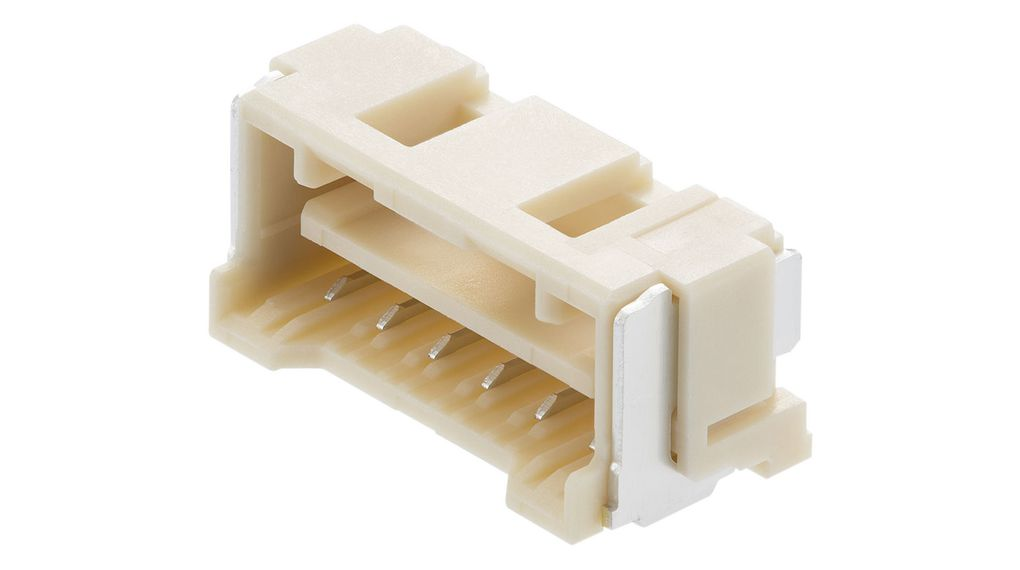
\includegraphics[scale=0.085]{./assets/figures/clik_mate.jpg}
    \caption{\cite{clikmate} Connecteur CLIK-Mate}
\end{figure}

En résumé, bien que le connecteur CLICK-Mate soit robuste, il est jugé trop grand et peu pratique à assembler.

\subsection{QWIIC}

Le connecteur QWIIC proposé par Sparkfun est compact.
En effet, pour un connecteur à quatre broches, la partie s'intégrant au circuit imprimé mesure 2,95 mm de hauteur, 6,25 mm de longueur et 7 mm de largeur.
Cependant, il peut être difficile de l'assembler soi-même sans l'outil approprié.
Il est préférable d'acheter des câbles pré-confectionnés, mais cela limite la possibilité de réaliser des câbles sur mesure sans avoir besoin de connecteurs supplémentaires.

\begin{figure}[H]
    \centering
    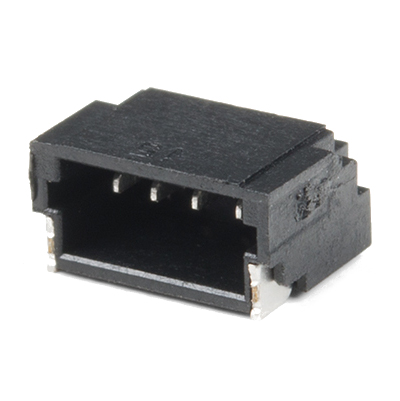
\includegraphics[scale=0.6]{./assets/figures/qwiic.jpg}
    \caption{\cite{qwiic} Connecteur QWIIC}
\end{figure}

En résumé, le connecteur QWIIC est compact mais peut être difficile à assembler sans l'outil approprié.

\subsection{Micro MaTch}

Le connecteur Micro MaTch, fabriqué par la société suisse TE Connectivity, présente l'avantage de pouvoir être assemblé manuellement avec des câbles plats.
En effet, les deux parties du connecteur viennent pincer le câble plat, établissant ainsi la connexion électrique.
La taille du connecteur pour quatre broches sur le circuit imprimé mesure 5,3 mm de hauteur, 6,9 mm de longueur et 9,7 mm de largeur.

\begin{figure}[H]
    \centering
    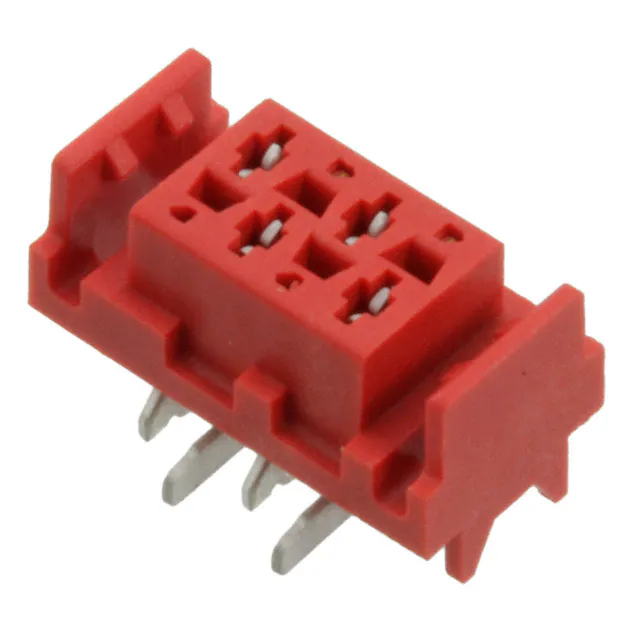
\includegraphics[scale=0.08]{./assets/figures/micromatch.png}
    \caption{\cite{micromatch} Connecteur Micro MaTch}
\end{figure}

En résumé, il est facile d'assembler le connecteur Micro MaTch à un câble plat, mais il n'est pas aussi compact que le connecteur QWIIC.

\subsection{Choix}

Le choix s'est porté sur le connecteur Micro MaTch.
En effet, il est facile à assembler manuellement et offre une compacité satisfaisante.
Bien qu'il soit légèrement moins compact que le connecteur QWIIC, cette différence ne pose pas de problème majeur.
Il est préférable d'avoir un connecteur légèrement plus grand en échange d'une meilleure solidité.
L'avantage principal du connecteur Micro MaTch est la possibilité de l'assembler manuellement sans avoir besoin d'un équipement spécifique.
La référence du connecteur Micro Match choisi est 338069-4.

Cependant, il est important de noter que le connecteur n'est pas un élément essentiel. Il peut être remplacé par un autre connecteur existant pour s'adapter à d'autres projets. Un minimum de 4 broches est nécessaire pour l'alimentation et l'I2C.

\section{Circuit imprimé}

La conception du circuit imprimé a été confiée à l'\gls{iai} de la \gls{heig}, afin de maintenir une conception interne offrant une flexibilité pour les modifications ultérieures.
Monsieur Luca Romano est la personne responsable de la conception et de la réalisation de la carte au sein de l'\gls{iai}. Cette approche vise également à maintenir une cohérence avec les autres projets de l'institut.
Le logiciel Altium Designer a été utilisé pour concevoir le circuit imprimé, en veillant à ce qu'il soit aussi compact que possible tout en facilitant la brasure.
Le circuit a été commandé chez Eurocircuit, et la brasure des composants a été réalisée par l'institut d'automatisation industrielle.

\section{Débogueur}

Il est possible d'effectuer la mise à jour du nouveau micrologiciel du microcontrôleur via le bus I2C.
Cependant, pour assurer son fonctionnement, il est nécessaire que le chargeur de démarrage préalablement développé dans le projet soit déjà présent.
Ainsi, il est nécessaire d'avoir un moyen d'implanter initialement le chargeur de démarrage sur le microcontrôleur.
À cette fin, il est nécessaire d'avoir un connecteur sur le circuit imprimé permettant d'accéder aux broches de programmation.
La marque \textit{Tag Connect} propose des solutions de câbles de connexion avec un connecteur directement intégré sur le circuit imprimé pour la programmation.
La solution choisie est le câble à six broches sans pattes, ce qui permet un encombrement minimal sur le circuit imprimé.
De plus, des adaptateurs du câble \textit{Tag Connect} vers le boîtier de programmation sont également disponibles.

\begin{figure}[H]
    \centering
    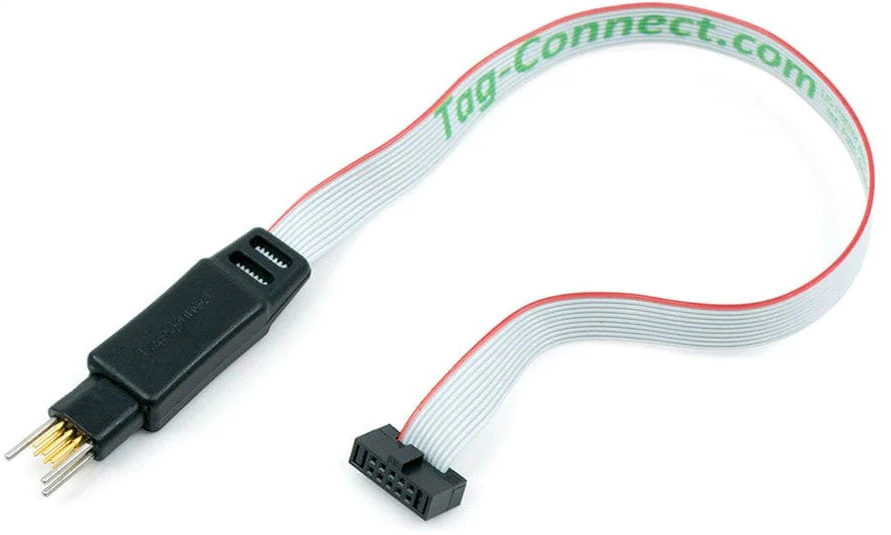
\includegraphics[scale=0.2]{./assets/figures/tag_connect.png}
    \caption{\cite{tag_connect} Câble Tag Connect six broches sans pattes}
\end{figure}

\begin{figure}[H]
    \centering
    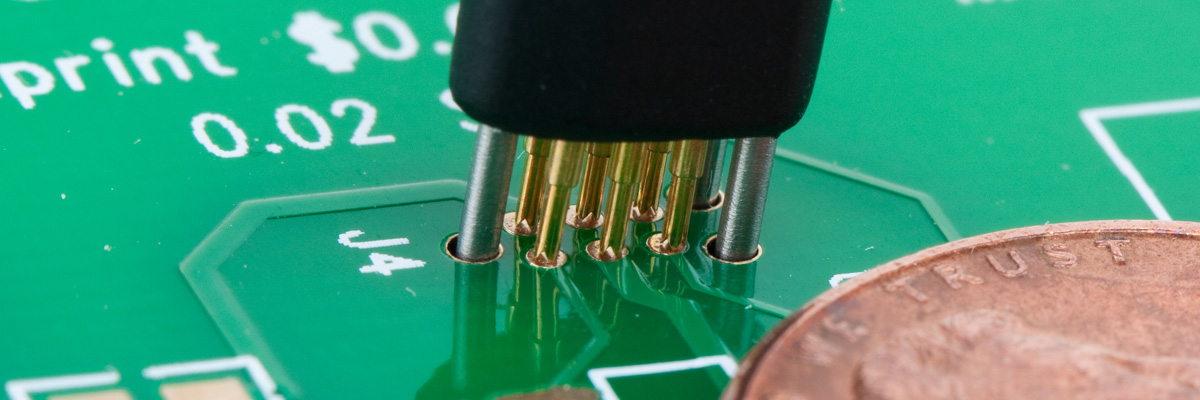
\includegraphics[scale=0.2]{./assets/figures/tag_connect_pcb.jpg}
    \caption{\cite{tag_connect_pcb} Câble Tag Connect six broches sans pattes connecté au circuit imprimé}
\end{figure}

De plus, un adaptateur est nécessaire pour établir une connexion ST-LINK avec l'ordinateur.
Le ST-LINK est un débogueur et programmateur pour les microcontrôleurs STM8 et STM32, qui assure la liaison entre l'ordinateur et le microcontrôleur.
Grâce à cette configuration, il est possible de programmer le chargeur de démarrage pour la première fois.

\begin{figure}[H]
    \centering
    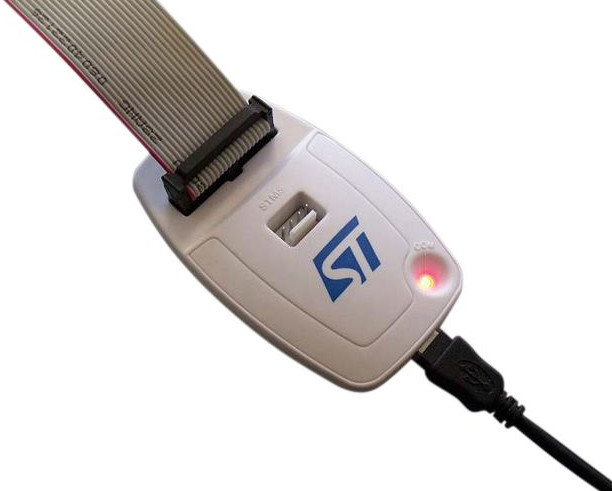
\includegraphics[scale=0.3]{./assets/figures/st_link.jpg}
    \caption{\cite{st_link} Débogueur et programmateur ST-LINK}
\end{figure}

Étant donné que le chargeur de démarrage doit être programmé une seule fois, il serait envisageable de le faire sur une partie fragile du circuit imprimé.
Ainsi, une fois programmé, cette partie fragile pourrait être retirée pour gagner de l'espace sur le circuit imprimé.
Cependant, cette approche n'a pas été utilisée dans le circuit imprimé réalisé, car la programmation du chargeur de démarrage sera réalisée à plusieurs reprises dans le cadre de ce projet.
Par conséquent, il est plus pratique de conserver le connecteur sur le circuit imprimé.

\section{Resistance}

Les équipements connectés à un bus I2C utilisent des sorties de type drain ouvert pour les deux lignes SDA et SCL.
L'état logique \textit{0} ou \textit{LOW} est l'état dominant, tandis que l'état logique \textit{1} ou \textit{HIGH} est l'état récessif.
Pour maintenir le bus à l'état de repos, des résistances de \textit{pull-up} sont utilisées pour le maintenir au niveau haut.

Par conséquent, il est nécessaire de mettre en place un système qui permet d'activer des résistances de \textit{pull-up} sur le dernier périphérique I2C.
Ce système doit être facile à activer ou désactiver, sachant que le changement de configuration se fera rarement.
Si possible, un système simple à braser serait préférable pour faciliter la mise en place de cette fonctionnalité.

Il a été décidé de mettre en place des pads qui permettent de réaliser un pont de soudure.
Lorsque le pont est établi, la résistance de \textit{pull-up} est activée.
L'avantage de ce système réside dans le fait qu'il ne nécessite aucun composant matériel supplémentaire.
De plus, le coût de ce pont de soudure est réduit.
Dans un système donné, le dernier périphérique peut varier, mais cela se produit rarement.
Par conséquent, le pont de soudure répond parfaitement à cette exigence et offre une solution simple et efficace pour activer les résistances de \textit{pull-up} lorsque cela est nécessaire.

\begin{figure}[H]
    \centering
    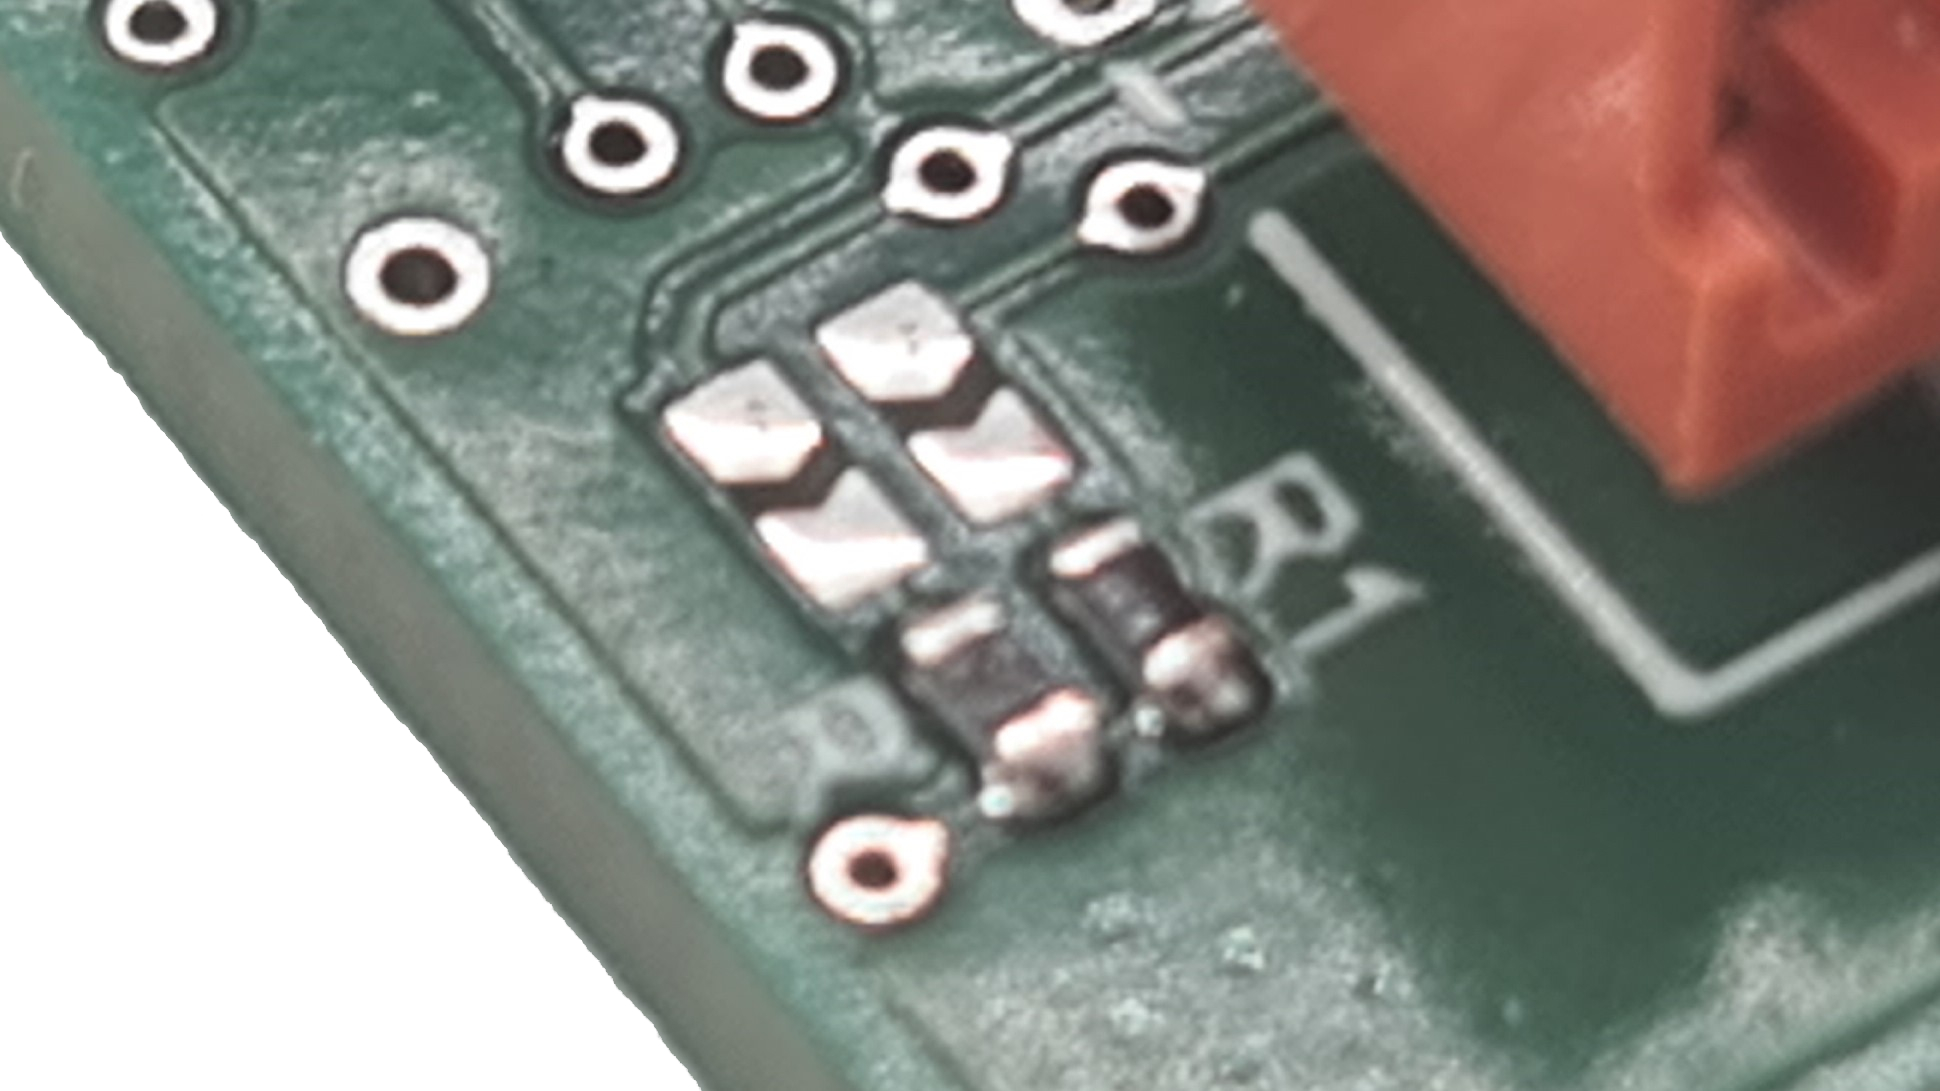
\includegraphics[scale=0.08]{./assets/figures/resistance_desactive.jpg}
    \caption{Résistances \textit{pull-up} non activées}
\end{figure}

\begin{figure}[H]
    \centering
    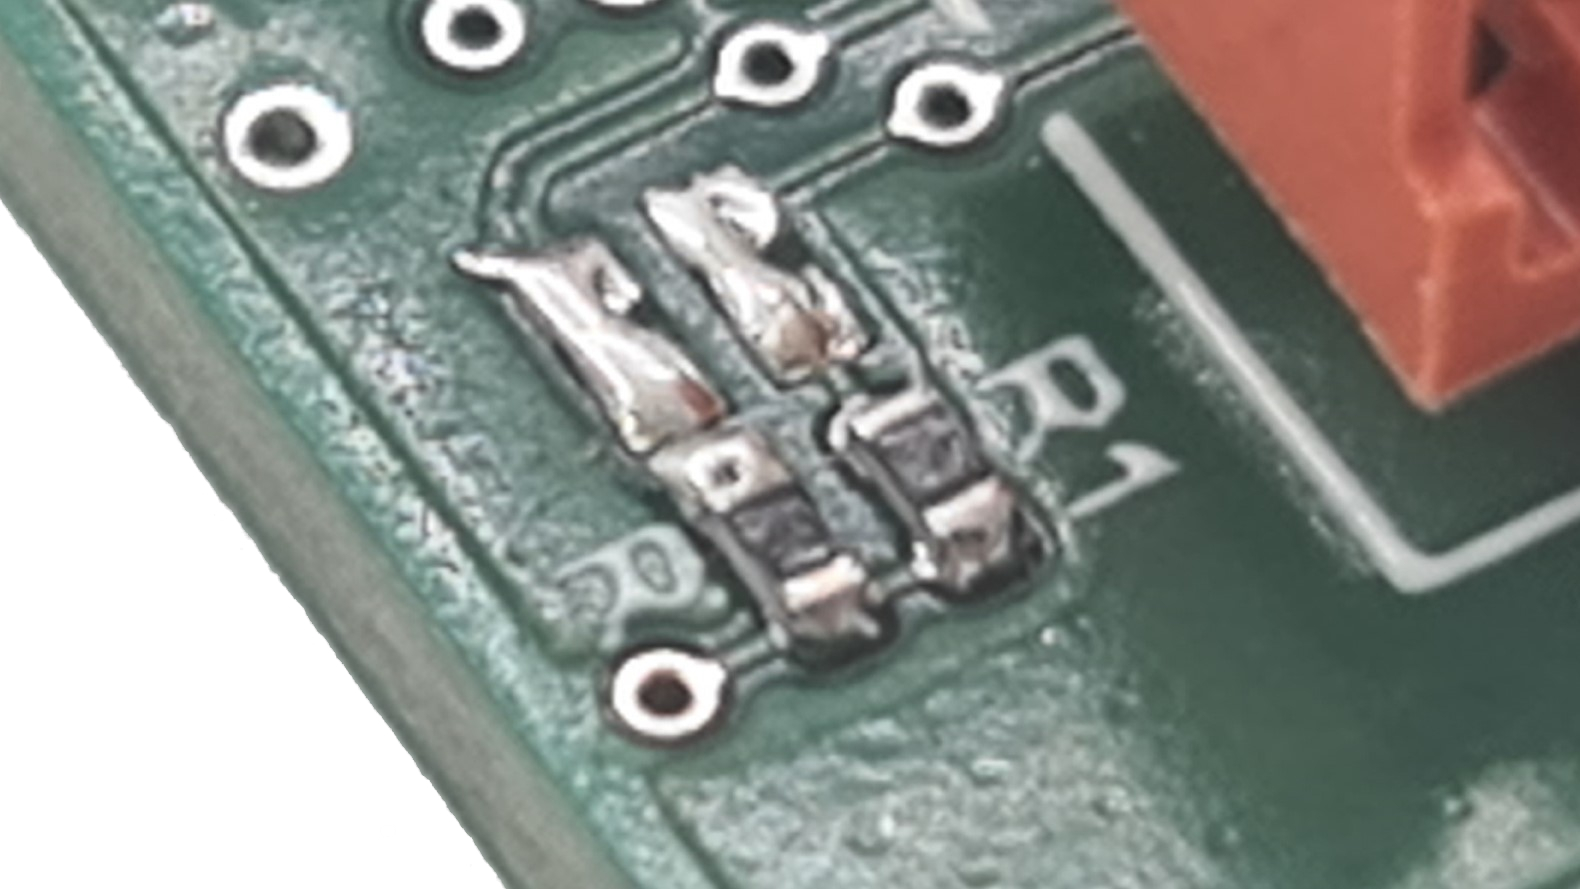
\includegraphics[scale=0.1]{./assets/figures/resistance_active.jpg}
    \caption{Résistances \textit{pull-up} activées}
\end{figure}

\section{Carte d'extension}

Pour se rapprocher au maximum d'une situation réelle, il est intéressant de mettre en place une carte d'extension pour le Raspberry Pi.
Cette carte d'extension permet d'utiliser le même connecteur que celui choisi sur la carte principale.
Ainsi, il est plus facile de connecter et déconnecter des périphériques plutôt que d'utiliser des câbles Dupont.
Il convient de souligner que cette carte d'extension n'est pas un circuit imprimé sophistiqué, mais simplement une plaque d'expérimentation (veroboard) équipée d'un connecteur et des connexions nécessaires.

\section{Tests}

Les tests matériels de la carte ont été effectués par l'\gls{iai}.
Lors de la livraison de la carte, il a été confirmé que les tests nécessaires au niveau matériel avaient été réalisés.
Par conséquent, la prochaine étape consiste à tester la partie logicielle du circuit imprimé pour s'assurer de son bon fonctionnement.

